\subsubsection{Общая информация об Apache Lucene, Solr}

Apache Solr - это расширяемая поисковая платформа от Apache. Система основана на библиотеке Apache Lucene и разработана на Java. Особенности ее в том, что она представляет из себя не просто техническое решение для поиска, а именно платформу, поведение которой можно легко расширять/менять/настраивать под любые нужды - от обычного полнотекстового поиска на сайте до распределенной системы хранения/получения/аналитики текстовых и других данных с мощным языком запросов. Lucene — самый известный из поисковых движков, изначально ориентированный именно на встраивание в другие программы.

\subsubsection{Подготовка окружения и установка Apache Lucene}
Добавление репозитория:
\textit
{
deb http://ppa.launchpad.net/webupd8team/java/ubuntu trusty main
deb-src http://ppa.launchpad.net/webupd8team/java/ubuntu trusty main
} (рис.~\ref{ship_9:ship_9}).

\begin{figure}[h!]
\center{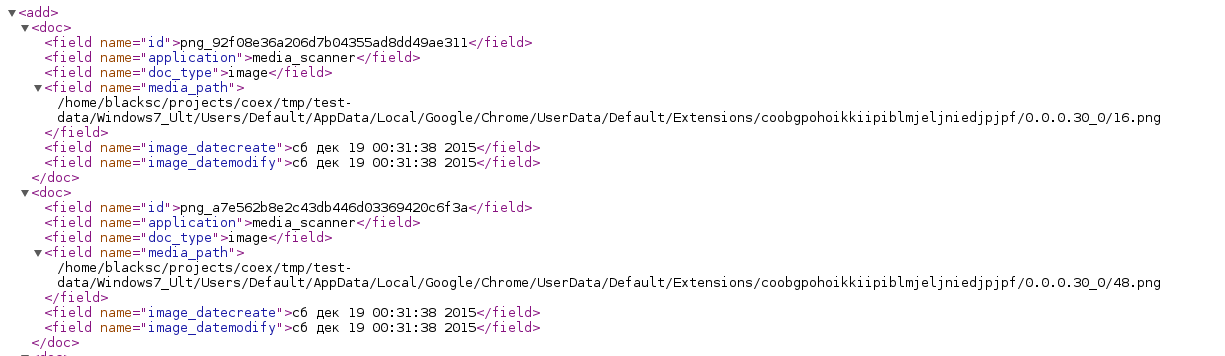
\includegraphics[width=1\linewidth]{ship_9}}
\caption{Добавление репозитория}
\label{ship_9:ship_9}
\end{figure}

Добавления ключа репозитория:
  \textit{
apt-key adv --keyserver hkp://keyserver.ubuntu.com:80 --recv-keys EEA14886
} (рис.~\ref{ship_10:ship_10}).

\begin{figure}[h!]
\center{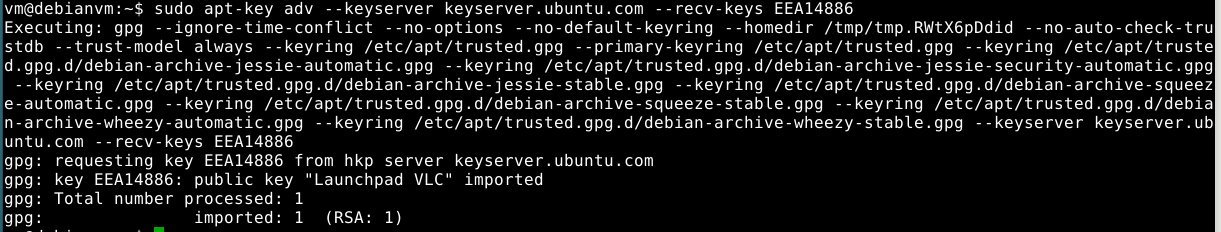
\includegraphics[width=1\linewidth]{ship_10}}
\caption{Добавление ключа}
\label{ship_10:ship_10}
\end{figure}

Обновление списка пакетов:
\textit
{
apt-get update
} (рис.~\ref{ship_11:ship_11}).

\begin{figure}[h!]
\center{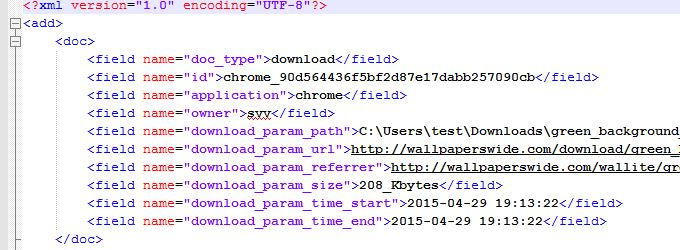
\includegraphics[width=1\linewidth]{ship_11}}
\caption{Обновление списка пакетов}
\label{ship_11:ship_11}
\end{figure}

Устанавка Java:
\textit
{
apt-get install oracle-java8-installer
} (рис.~\ref{ship_12:ship_12}).

\begin{figure}[h!]
\center{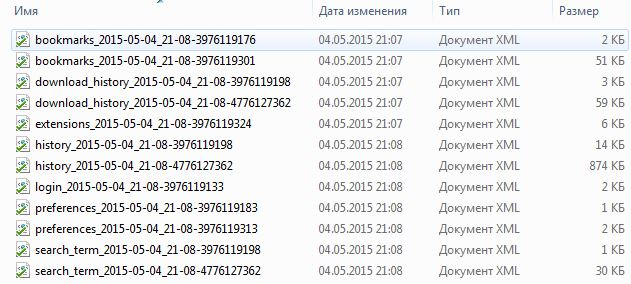
\includegraphics[width=1\linewidth]{ship_12}}
\caption{Установка java}
\label{ship_12:ship_12}
\end{figure}

Загрузка Apache Solr:
\textit
{
wget http://apache.mirror1.spango.com/lucene/solr/5.2.1/solr-5.2.1.tgz
} (рис.~\ref{ship_13:ship_13}).

\begin{figure}[h!]
\center{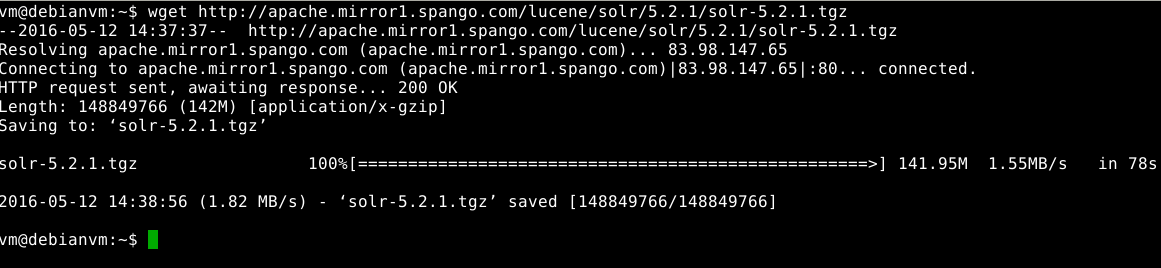
\includegraphics[width=1\linewidth]{ship_13}}
\caption{Загрузка Apache Solr}
\label{ship_13:ship_13}
\end{figure}

Распаковка архива и установка: 
\textit
{
tar xzf solr-5.2.1.tgz solr-5.2.1/bin/install\_solr\_service.sh --strip-components=2
}.
Устанавка Apache Solr командой 
\textit
{
sudo bash ./install\_solr\_service.sh solr-5.2.1.tgz
} (рис.~\ref{ship_14:ship_14}).
\begin{figure}[h!]
\center{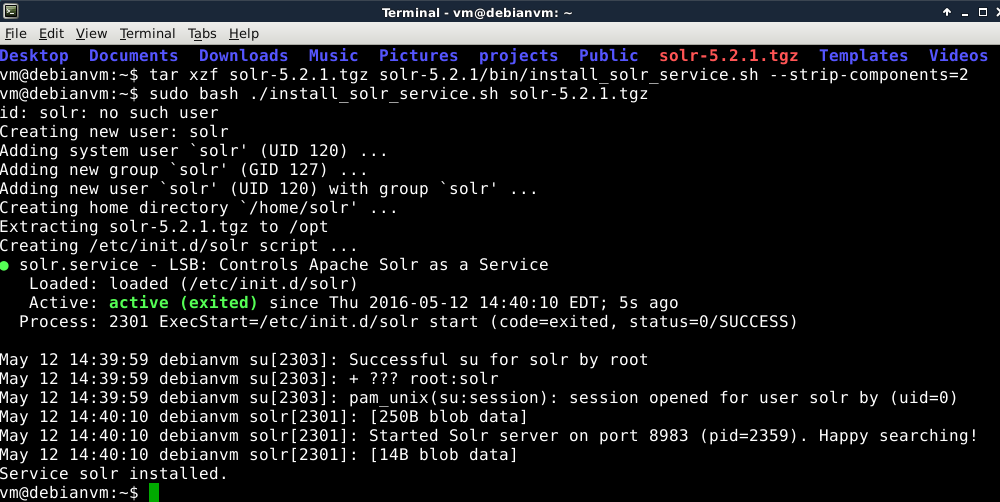
\includegraphics[width=1\linewidth]{ship_14}}
\caption{Распаковка и установка}
\label{ship_14:ship_14}
\end{figure}

Apache Solr по умолчанию работает на порту 8983. Проверка работоспособности в браузере (рис.~\ref{ship_15:ship_15}).

\begin{figure}[h!]
\center{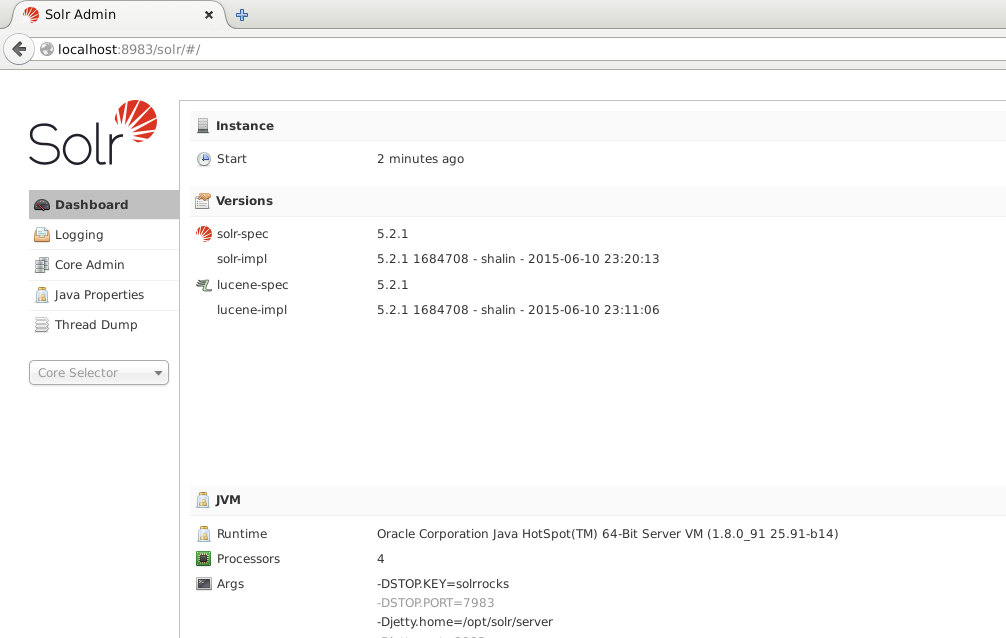
\includegraphics[width=1\linewidth]{ship_15}}
\caption{Проверка работоспособности Apache Solr}
\label{ship_15:ship_15}
\end{figure}

\subsubsection{Добавление документов в поисковый индекс}

Solr запущен, но на данный момент он не содержит каких-либо данных в поисковом индексе. 
Для отправки данных на сервер воспользуется shell скриптом, который будет брать содержимое XML файлов из необходимой директории и отправлять их Solr. В результате произошло добавления документов в Solr. Solr, в отличие от других систем хранит не документ целиком и выполняет поиск по нему, а разбивает XML-документ на поля и индексирует каждое из них  (рис.~\ref{ship_16:ship_16}).

\begin{figure}[h!]
\center{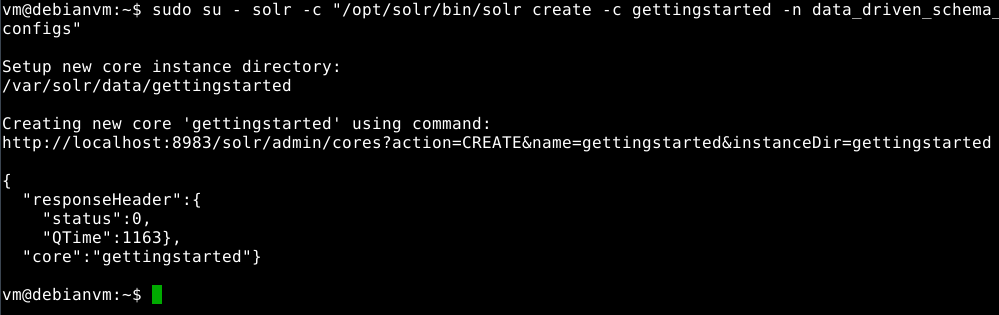
\includegraphics[width=1\linewidth]{ship_16}}
\caption{Загрузка документов}
\label{ship_16:ship_16}
\end{figure}

\subsubsection{Формирование запросов}
Так как документ в поисковом индексе представляет собой набор полей, то возможно формировать сложные поисковые запросы, которые при выполнении используют значения отдельных полей документа (рис.~\ref{ship_18:ship_18}). 

\begin{figure}[h!]
\center{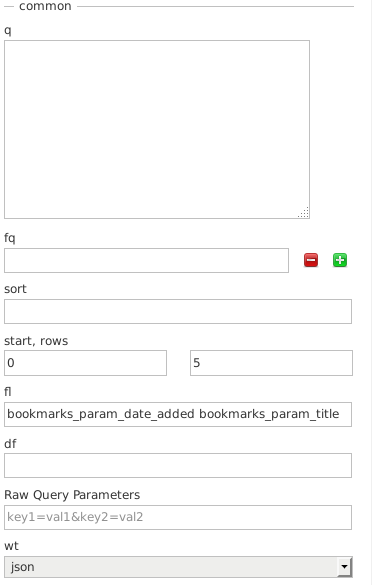
\includegraphics[width=0.4\linewidth]{ship_18}}
\caption{Область ввода запросов}
\label{ship_18:ship_18}
\end{figure}

В области для ввода запросов присутсвуют следующие поля:
\begin{enumerate}
  \item q - основной запрос;
  \item fq - фильтрующий запрос;
  \item start - сдвиг в поиске;
  \item rows - кол-во выводимых результатов;
  \item fl - выводимые поля;
  \item wt - формат вывода данных.
\end{enumerate}

Примеры запросов:
\begin{enumerate}
  \item по содержанию значения в каком-либо поле документа (рисунок ~\ref{ship_19:ship_19});
  \item по содержанию в поле определенного значения (рисунок ~\ref{ship_20:ship_20});
  \item по значению поля, находящемуся в определенном интервале (рисунок~\ref{ship_21:ship_21}, рисунок ~\ref{ship_22:ship_22}), с использованием вывода конкретных полей (рисунок~\ref{ship_23:ship_23});
  \item с использованием булевых операторов (рисунок~\ref{ship_24:ship_24}).
\end{enumerate}

\begin{figure}[h!]
\center{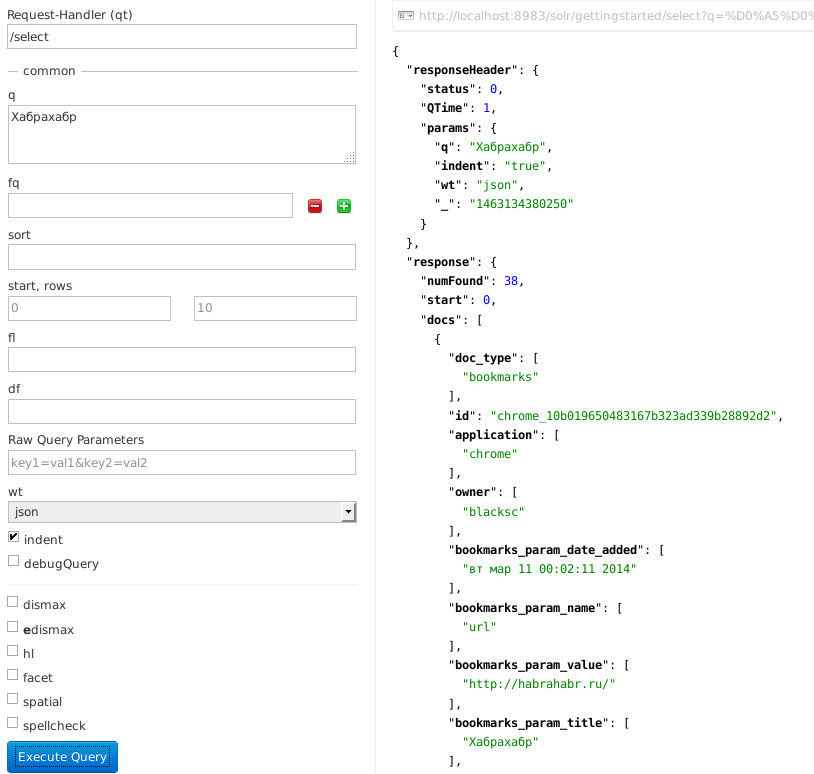
\includegraphics[width=0.7\linewidth]{ship_19}}
\caption{Запрос по содержанию в каком-либо поле документа}
\label{ship_19:ship_19}
\end{figure}

\begin{figure}[h!]
\center{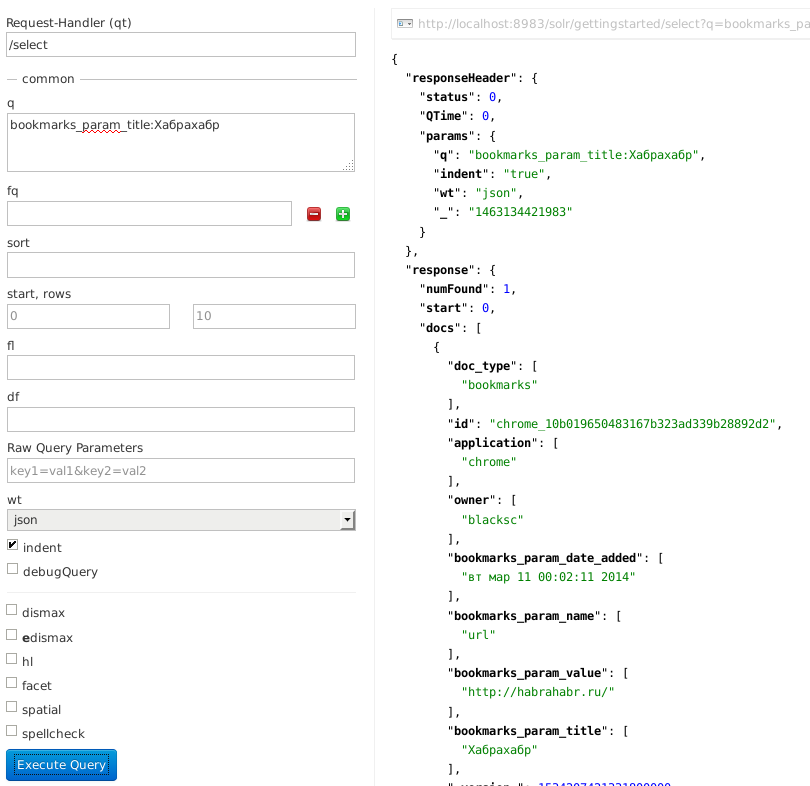
\includegraphics[width=1\linewidth]{ship_20}}
\caption{Запрос по содержанию в поле определенного значения}
\label{ship_20:ship_20}
\end{figure}

\begin{figure}[h!]
\center{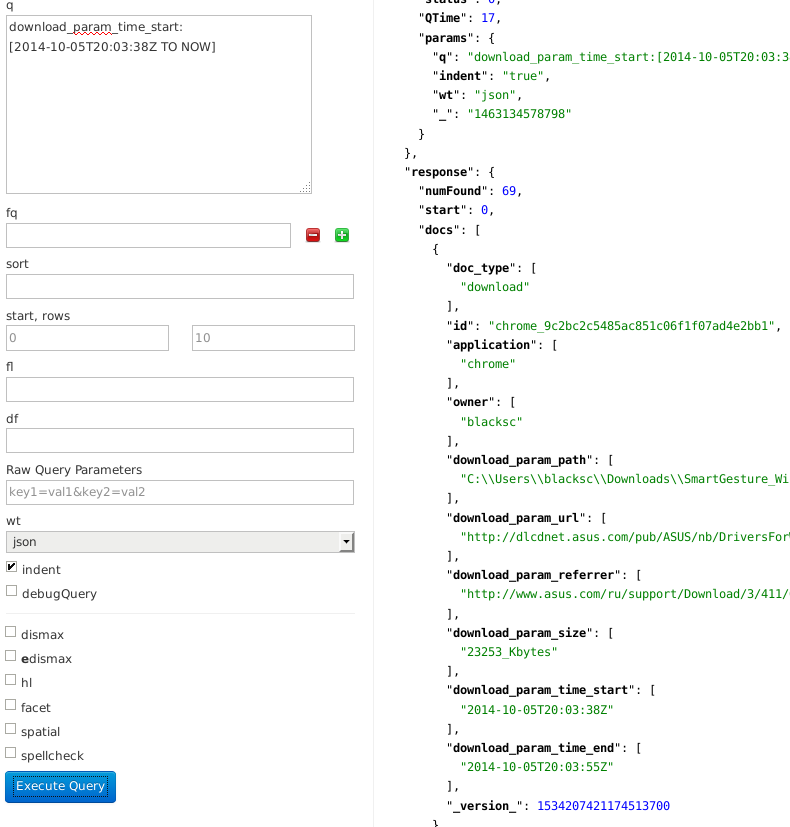
\includegraphics[width=1\linewidth]{ship_21}}
\caption{Запрос по значению поля даты, находящиеся в интервале от определенного значения до настоящего времени}
\label{ship_21:ship_21}
\end{figure}

\begin{figure}[h!]
\center{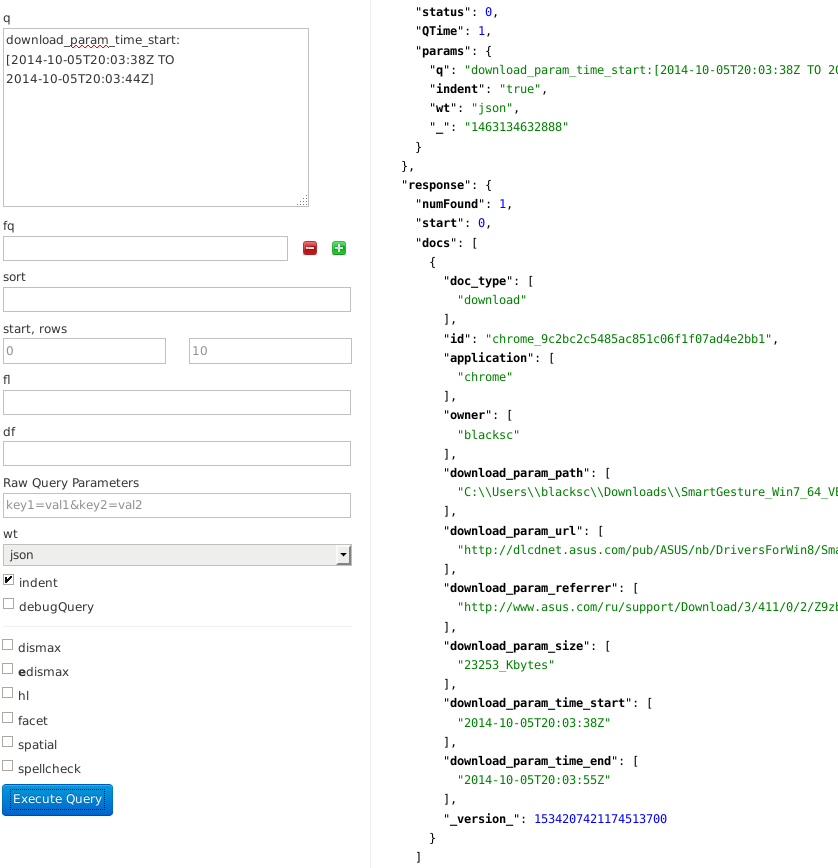
\includegraphics[width=1\linewidth]{ship_22}}
\caption{Запрос по значению поля даты, находящемуся в определенном интервале}
\label{ship_22:ship_22}
\end{figure}


\begin{figure}[h!]
\center{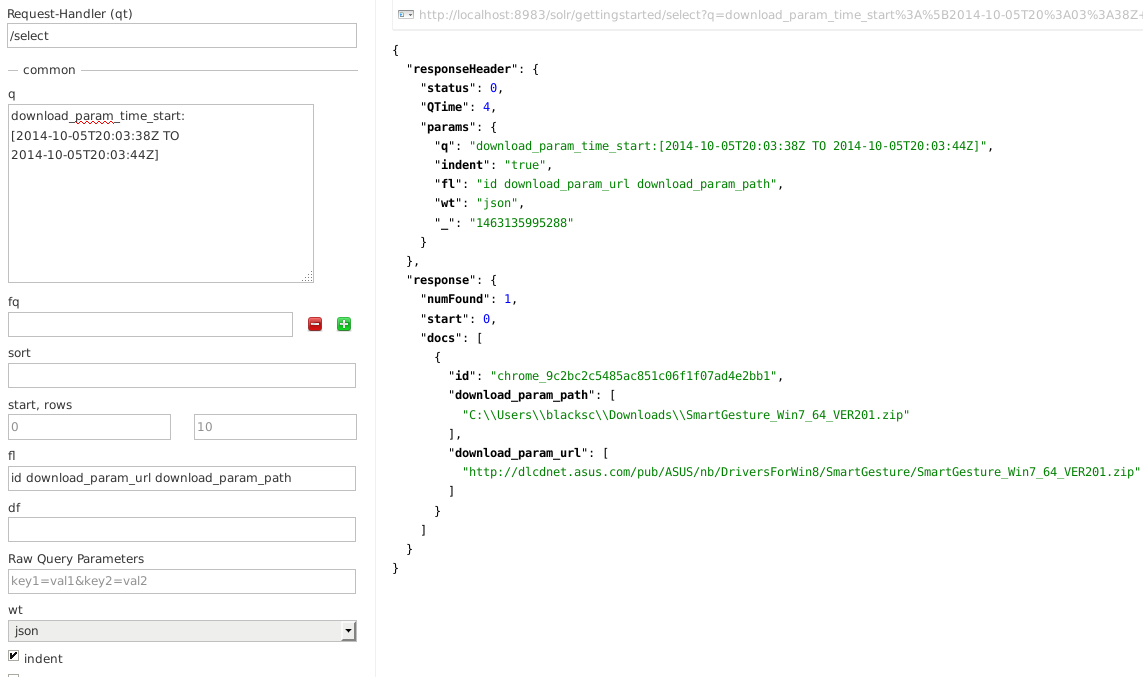
\includegraphics[width=1\linewidth]{ship_23}}
\caption{Запрос с выводом определенных полей}
\label{ship_23:ship_23}
\end{figure}

\begin{figure}[h!]
\center{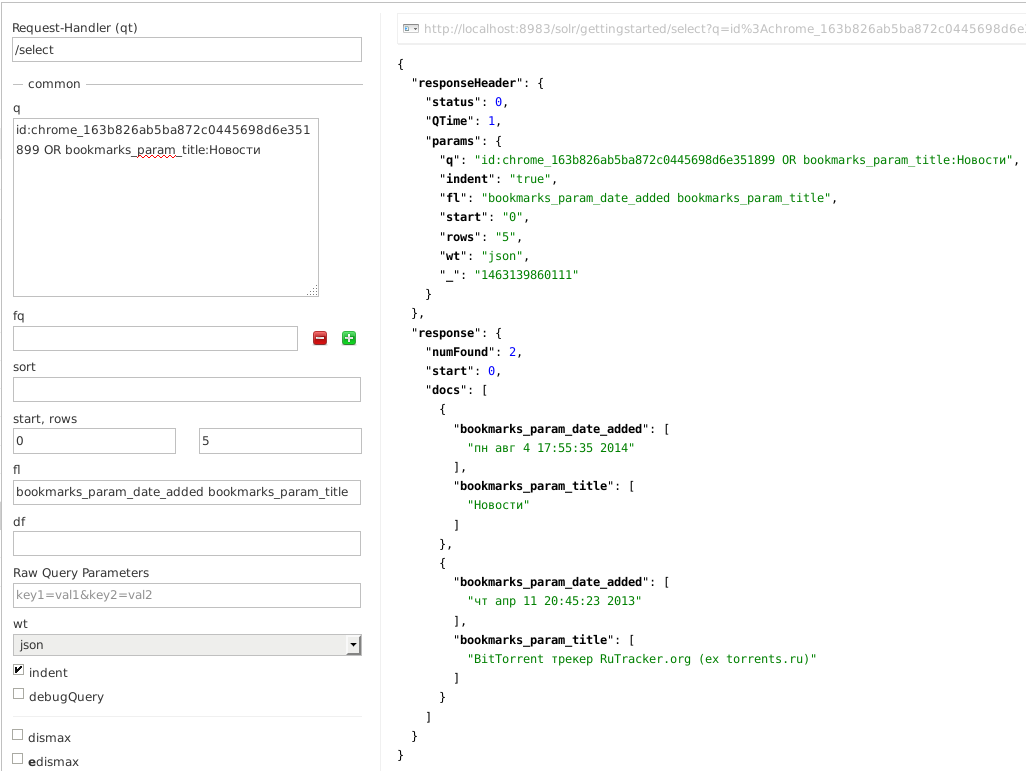
\includegraphics[width=1\linewidth]{ship_24}}
\caption{Запрос с использованием булевого оператора}
\label{ship_24:ship_24}
\end{figure}

\clearpage
